\documentclass[10pt,a4paper]{article}
\usepackage[utf8]{inputenc}
\usepackage{amsfonts}
\usepackage{amssymb}
\usepackage{float}
\usepackage{graphicx}
\usepackage{wrapfig}
\date{}
\title{Welcome to Paperwork !}
\setlength{\parskip}{\baselineskip}%

\begin{document}
\maketitle

\begin{figure}[h]
	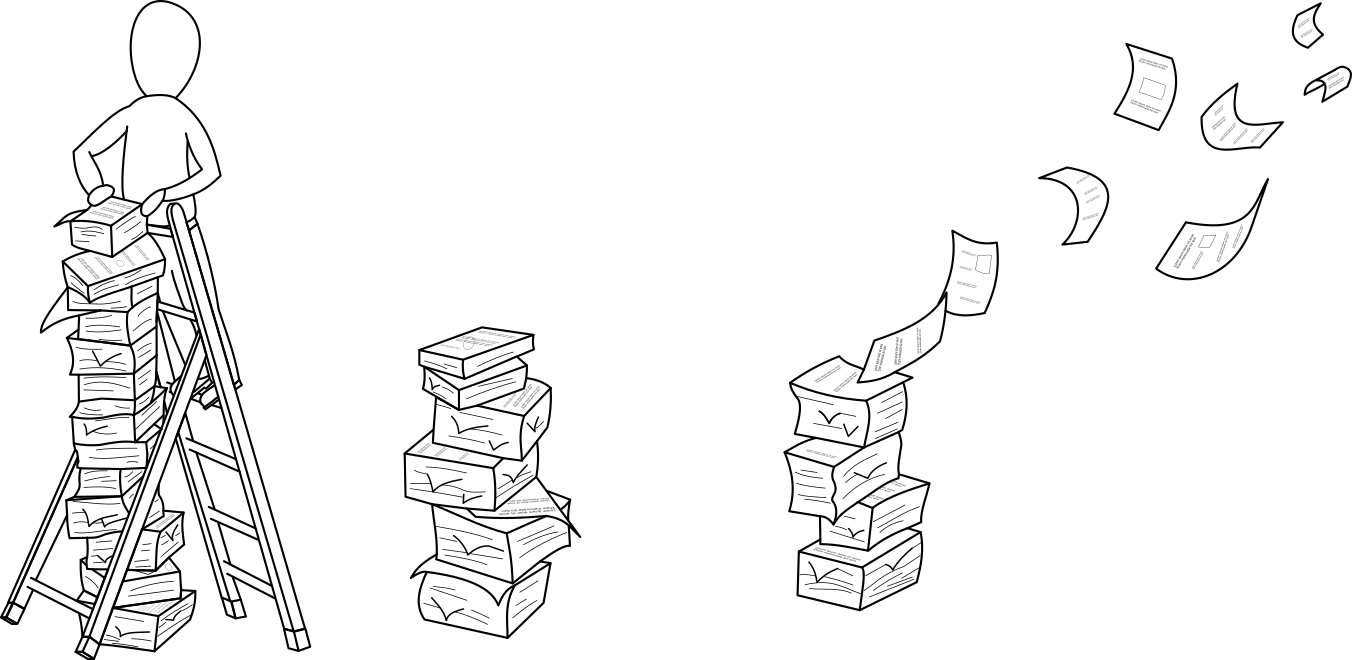
\includegraphics[width=\linewidth]{data/intro.png}
\end{figure}

They are going to drive you crazy. Your phone operator, your bank, your daughter's school, your dog's veterinarian, even your ISP; it seems like all of them are trying to drown you under tons of papers. Papers you have to read, classify, and memorize just in case you may need them later. Most of the time you won't, which means you waste your energy for nothing.

Paperwork will help you get rid of all those papers by turning them into searchable documents.
It's simple: just scan and forget. Looking for a specific paper?
Just type in a few keywords and tada

\pagebreak

\section{Documents and pages}

\begin{figure}[h]
	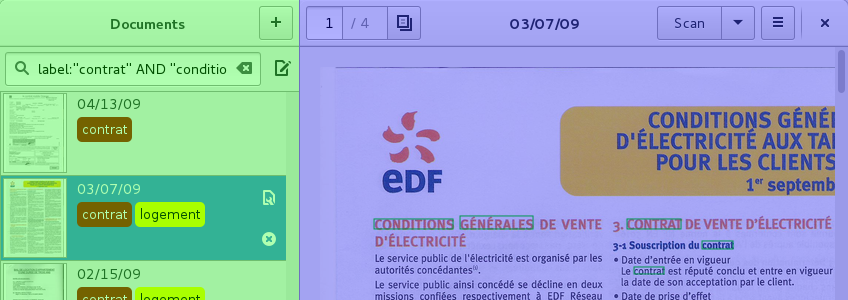
\includegraphics[width=\linewidth]{data/paperwork_main_window_split.png}
\end{figure}

Paperwork's interface is composed of two panels. On the left (green) is the
list of all your documents sorted by the date they were imported. On the right
(blue) are the pages of the currently selected paper.

You can add papers from several sources, depending on the devices connected
to your computer: scanner flatbed, scanner feeder, camera, etc. You have no
scanner at home? You can still use the scanner you have at work. Paperwork
will easily import PDF and image files.


\section{Find}

\begin{wrapfigure}{r}{0.5\textwidth}
	\centering
	\vspace{-20pt}
	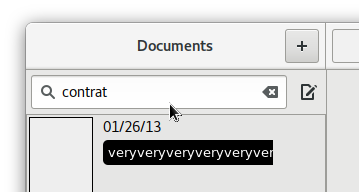
\includegraphics[scale=0.5]{data/paperwork_search.png}
\end{wrapfigure}

Find what you need, when you need it. Type a few keywords in the search
bar and the list of papers will shrink to only the relevant content. This
is where the magic happens: Paperwork uses optical character recognition
(OCR) to convert your papers into simple text files, so it's easy to
search for text.


\section{Export}

\begin{figure}[h]
	\centering
	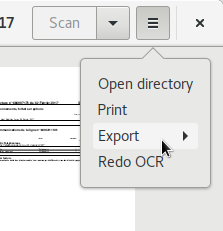
\includegraphics[scale=0.5]{data/paperwork_export_0001.png}
	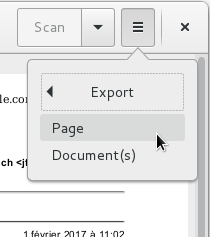
\includegraphics[scale=0.5]{data/paperwork_export_0002.png}
\end{figure}

Sometimes you may want to export a document to send it to someone else.
Multiple formats are supported: .pdf, .jpg, .txt, etc. And of course, paper
(requires a printer, sold separately).


\section{Labels and additional keywords}

\begin{figure}[h]
	\centering
	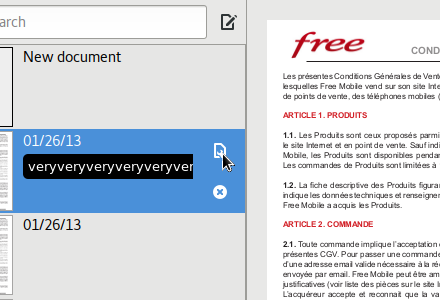
\includegraphics[scale=0.3]{data/paperwork_goto_labels_and_memo.png}
	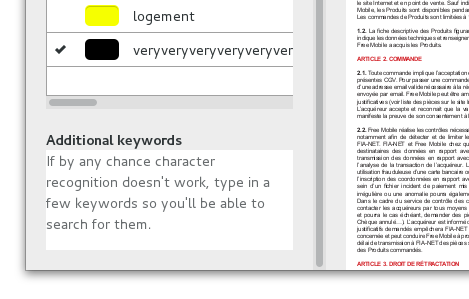
\includegraphics[scale=0.3]{data/paperwork_label_and_memo.png}
\end{figure}

You answered an important email and you want to keep track of it? The paper
you scanned was so unreadable that Paperwork failed to recognize some impor-
tant keywords? Add keywords to your paper so you won't miss anything! All
the keywords you add will be searchable, as if they were directly written on
the paper you scanned.

You would like to organize your documents a bit more? You can also add labels
to your documents. Each label has its own color. With time, Paperwork will
learn which labels go on which documents and will automatically apply them
on new documents.


\section{Your first documents}

\begin{figure}[h]
	\centering
	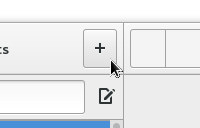
\includegraphics[scale=0.5]{data/new_doc.png}
	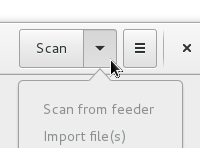
\includegraphics[scale=0.5]{data/paperwork_import.png}
	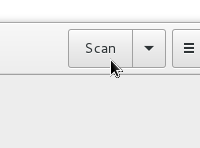
\includegraphics[scale=0.5]{data/paperwork_scan.png}
\end{figure}

Click the + button, the scan button, and that's all folks! You are now aware
of the main features of Paperwork. You can start using it by adding your first
own paper.


\section{Need more help ?}

\begin{figure}[H]
	\centering
	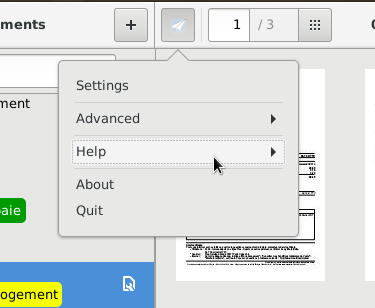
\includegraphics[scale=0.33]{data/menu_help.png}
	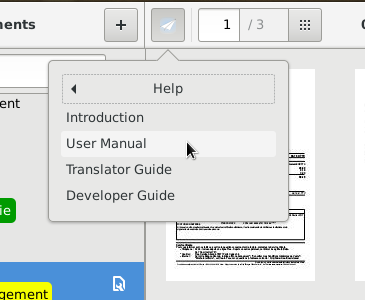
\includegraphics[scale=0.33]{data/menu_help_user_manual.png}
\end{figure}

If you need more help, there is a comprehensive manual you can find in the help
section of Paperwork.

We hope that you'll enjoy this piece of software. If you like it please tell
us, and if you don't please tell us why!

\begin{figure}[b]
	
\includegraphics[width=\linewidth]{data/paperwork_going_up.png}
\end{figure}

\end{document}
